%%%%%%%%%%%%%%%%%%%%%%%%%%%%%%%%%%%%%%%%%%%%%%%%%%%%%%%%%%%%%%%%%%%%%%%
% BAB 4
%%%%%%%%%%%%%%%%%%%%%%%%%%%%%%%%%%%%%%%%%%%%%%%%%%%%%%%%%%%%%%%%%%%%%%%

\mychapter{4}{BAB 4 METODOLOGI}

Bab ini menjelaskan tentang langkah-langkah yang dilakukan selama
pengembangan pengujian. Setelah studi literatur selesai dilakukan,
dilaksanakan proses analisis kebutuhan pengujian, perencanaan dan
implementasi kasus uji, dan penarikan kesimpulan.

\begin{figure}[H]
  \centering
  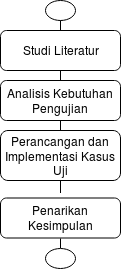
\includegraphics[width=.2\linewidth]{img/diagram-uji3}
  \caption{Alur metodologi}
  \label{fig:alur-metodologi}
\end{figure}

\section{Studi Literatur}

Studi Literatur dibutuhkan untuk mendalami teori-teori tentang
pengujian lebih dalam. Sumber dari literatur tersebut berasal dari
jurnal, buku, situs resmi maupun buku panduan perangkat lunak
yang digunakan. Daftar literatur yang didalami terkait dengan:

\begin{enumerate}
\item Penelitian-penelitian terkait pengujian
\item Metode-metode pengujian yaitu \emph{white-box} dan \emph{black-box}.
\item Tahapan pengujian \emph{unit} dan \emph{integration}.
\item Teknik pengujian \emph{basis path testing, boundary value
    analysis} dan \emph{ equivalence partitioning}.
\item Teknologi yang digunakan dalam penelitian
\end{enumerate}

\section{Analisis Kebutuhan Pengujian}

Pada proses analis kebutuhan pengujian akan ditentukan tahapan yang
akan di lakukan dan bagian yang akan diuji. Pengujian pada
\emph{neo-cli} hanya dilakukan hanya pada tahapan \emph{unit} dan
\emph{integration}.  Pada fase ini ditentukan juga \emph{method}
apa saja yang akan diuji. Penentuan tahapan pengujian dan penetuan
\emph{method} yang akan diuji dilakukan oleh pembimbing lapangan
dengan beberapa pertimbangan. Di antara pertimbangan tersebut adalah
waktu praktik kerja lapangan yang terbatas.

\section{Perancangan dan Implementasi Kasus Uji}

Pada proses ini dilakukan perancangan dan implementasi (eksekusi)
kasus uji. Tahapan yang dilakukan diawali dengan pengujian \emph{unit}
kemudian pengujian \emph{integration}. Metode pengujian yang digunakan
adalah metode pengujian \emph{white-box} dan metode pengujian
\emph{black-box}. Teknik yang digunakan selama proses pengujian dengan
methode \emph{white-box} adalah teknik \emph{basis path testing}.
Teknik \emph{equivalence partitioning} dan \emph{boundary value
  analysis} adalah teknik yang digunakan selama proses pengujian
dengan metode \emph{black-box}. Perancangan kasus uji dalam metode
\emph{white-box} diawali dengan pembuatan \emph{flow graph} dari
sebuah \emph{pseudocode}, kemudian menghitung \emph{cyclomatic
  complexity}, menentukan \emph{independent path} dan merancang kasus
uji sesuai dengan \emph{idependent path} yang didapatkan. Sedangkan
perancangan kasus uji pada metode \emph{black-box} didapatkan dari
data pengujian yang dihasilkan dari penggunaan teknik
\emph{equivalence partitioning} dan \emph{boundary value analysis}.
Implementasi pengujian atau eksekusi pengujian dilakukan secara
langsung setelah perancangan pada tahapan \emph{unit} dan
\emph{integration} selesai. Hasil dari implementasi tersebut juga
langsung dipaparkan. Hasil dari implementasi atau eksekusi pengujian
diletakkan pada kolom \emph{result} dan \emph{status} pada tabel kasus
uji. Metode pengujian \emph{white-box} dilakukan pada seluruh tahapan
\emph{unit} dan \emph{integration}. Sedangkan metode pengujian
\emph{black-box} hanya dilakukan pada bagian integrasi sistem yang
meminta masukan kepada pengguna, seperti yang terjadi pada
\emph{method do\_login}. Setelah pengujian secara manual pada tahap
\emph{unit} dan \emph{integration} selesai dilakukan, maka dibangun
\emph{test script} untuk \emph{automated testing} sehingga proses
pengujian selanjutnya dapat dilakukan secara otomatis. \emph{Automated
  testing} dilakukan menggunakan bantuan kakas bantu \emph{travis-ci}
yang konfigurasinya dijelaskan pada subbab ``Pengaturan Lingkungan
Pengujian untuk \emph{Automated Testing}''. Perhitungan cakupan
pengujian dilakukan dengan bantuan kakas bantu \emph{coverage.py} yang
hasil cakupannya dijelaskan pada subbab ``Hasil Cakupan Pengujian''.

\section{Penarikan Kesimpulan}

Pengujian ditutup setelah semua \emph{method} pada analisis kebutuhan
pengujian selesai diuji. Penarikan kesimpulan dilakukan setelah
pengujian ditutup. Kesimpulan diambil berdasarkan hasil dari seluruh
proses yang dilakukan selama pengujian. Kesalahan-kesalahan akan dicat
dan dijadikan saran agar tidak terulang kembali pada proses pengujian
selanjutnya. Kesimpulan pengujian nantinya dapat digunakan untuk
perbaikan dan peningkatan pengujian-pengujian selanjutnya.

%%% Local Variables:
%%% mode: latex
%%% TeX-master: "pkl"
%%% End:
